\documentclass[11pt]{beamer}
\usetheme{Goettingen}
\usepackage[utf8]{inputenc}
\usepackage{amsmath}
\usepackage{amsfonts}
\usepackage{amssymb}
\usepackage{xfrac}
\usepackage{graphicx}
\usepackage{caption}
\usepackage{enumerate}
\usepackage{enumitem}
\usepackage{xcolor}
\usepackage{inputenc}

\makeatletter
\newenvironment<>{proofs}[1][\proofname]{%
    \par
    \def\insertproofname{#1\@addpunct{.}}%
    \usebeamertemplate{proof begin}#2}
  {\usebeamertemplate{proof end}}
\makeatother

\newtheorem{proposition}{Proposition}[section]
\newcommand{\pr}{{\rm Pr}}
\newcommand{\e}{{\rm E}}
\newcommand{\expdist}{{\rm exp}}
\newcommand{\U}{{\rm U}}
\DeclareMathOperator*{\argmin}{arg\,min}

\author{Ran Snitkovsky}
\title{Strategic Sensing in Cognitive Radio Networks}
\setbeamercovered{transparent} 
%\setbeamertemplate{navigation symbols}{} 

\institute{\scriptsize 
 Under Supervision of \\ \normalsize Prof.~Refael Hassin \\ \bigskip \scriptsize The Raymond and Beverly Sackler Faculty of Exact Sciences\\ The Department of Statistics and Operations Research\\ Tel-Aviv University} 
\date{September 26, 2015} 
\subject{Equilibrium Behavior in Queueing Systems}
\begin{document}

\begin{frame}
\titlepage
\end{frame}

\begin{frame}{Introduction}\pause
The problem: 
\visible<3>{
\begin{figure}[h!]
  \centering
   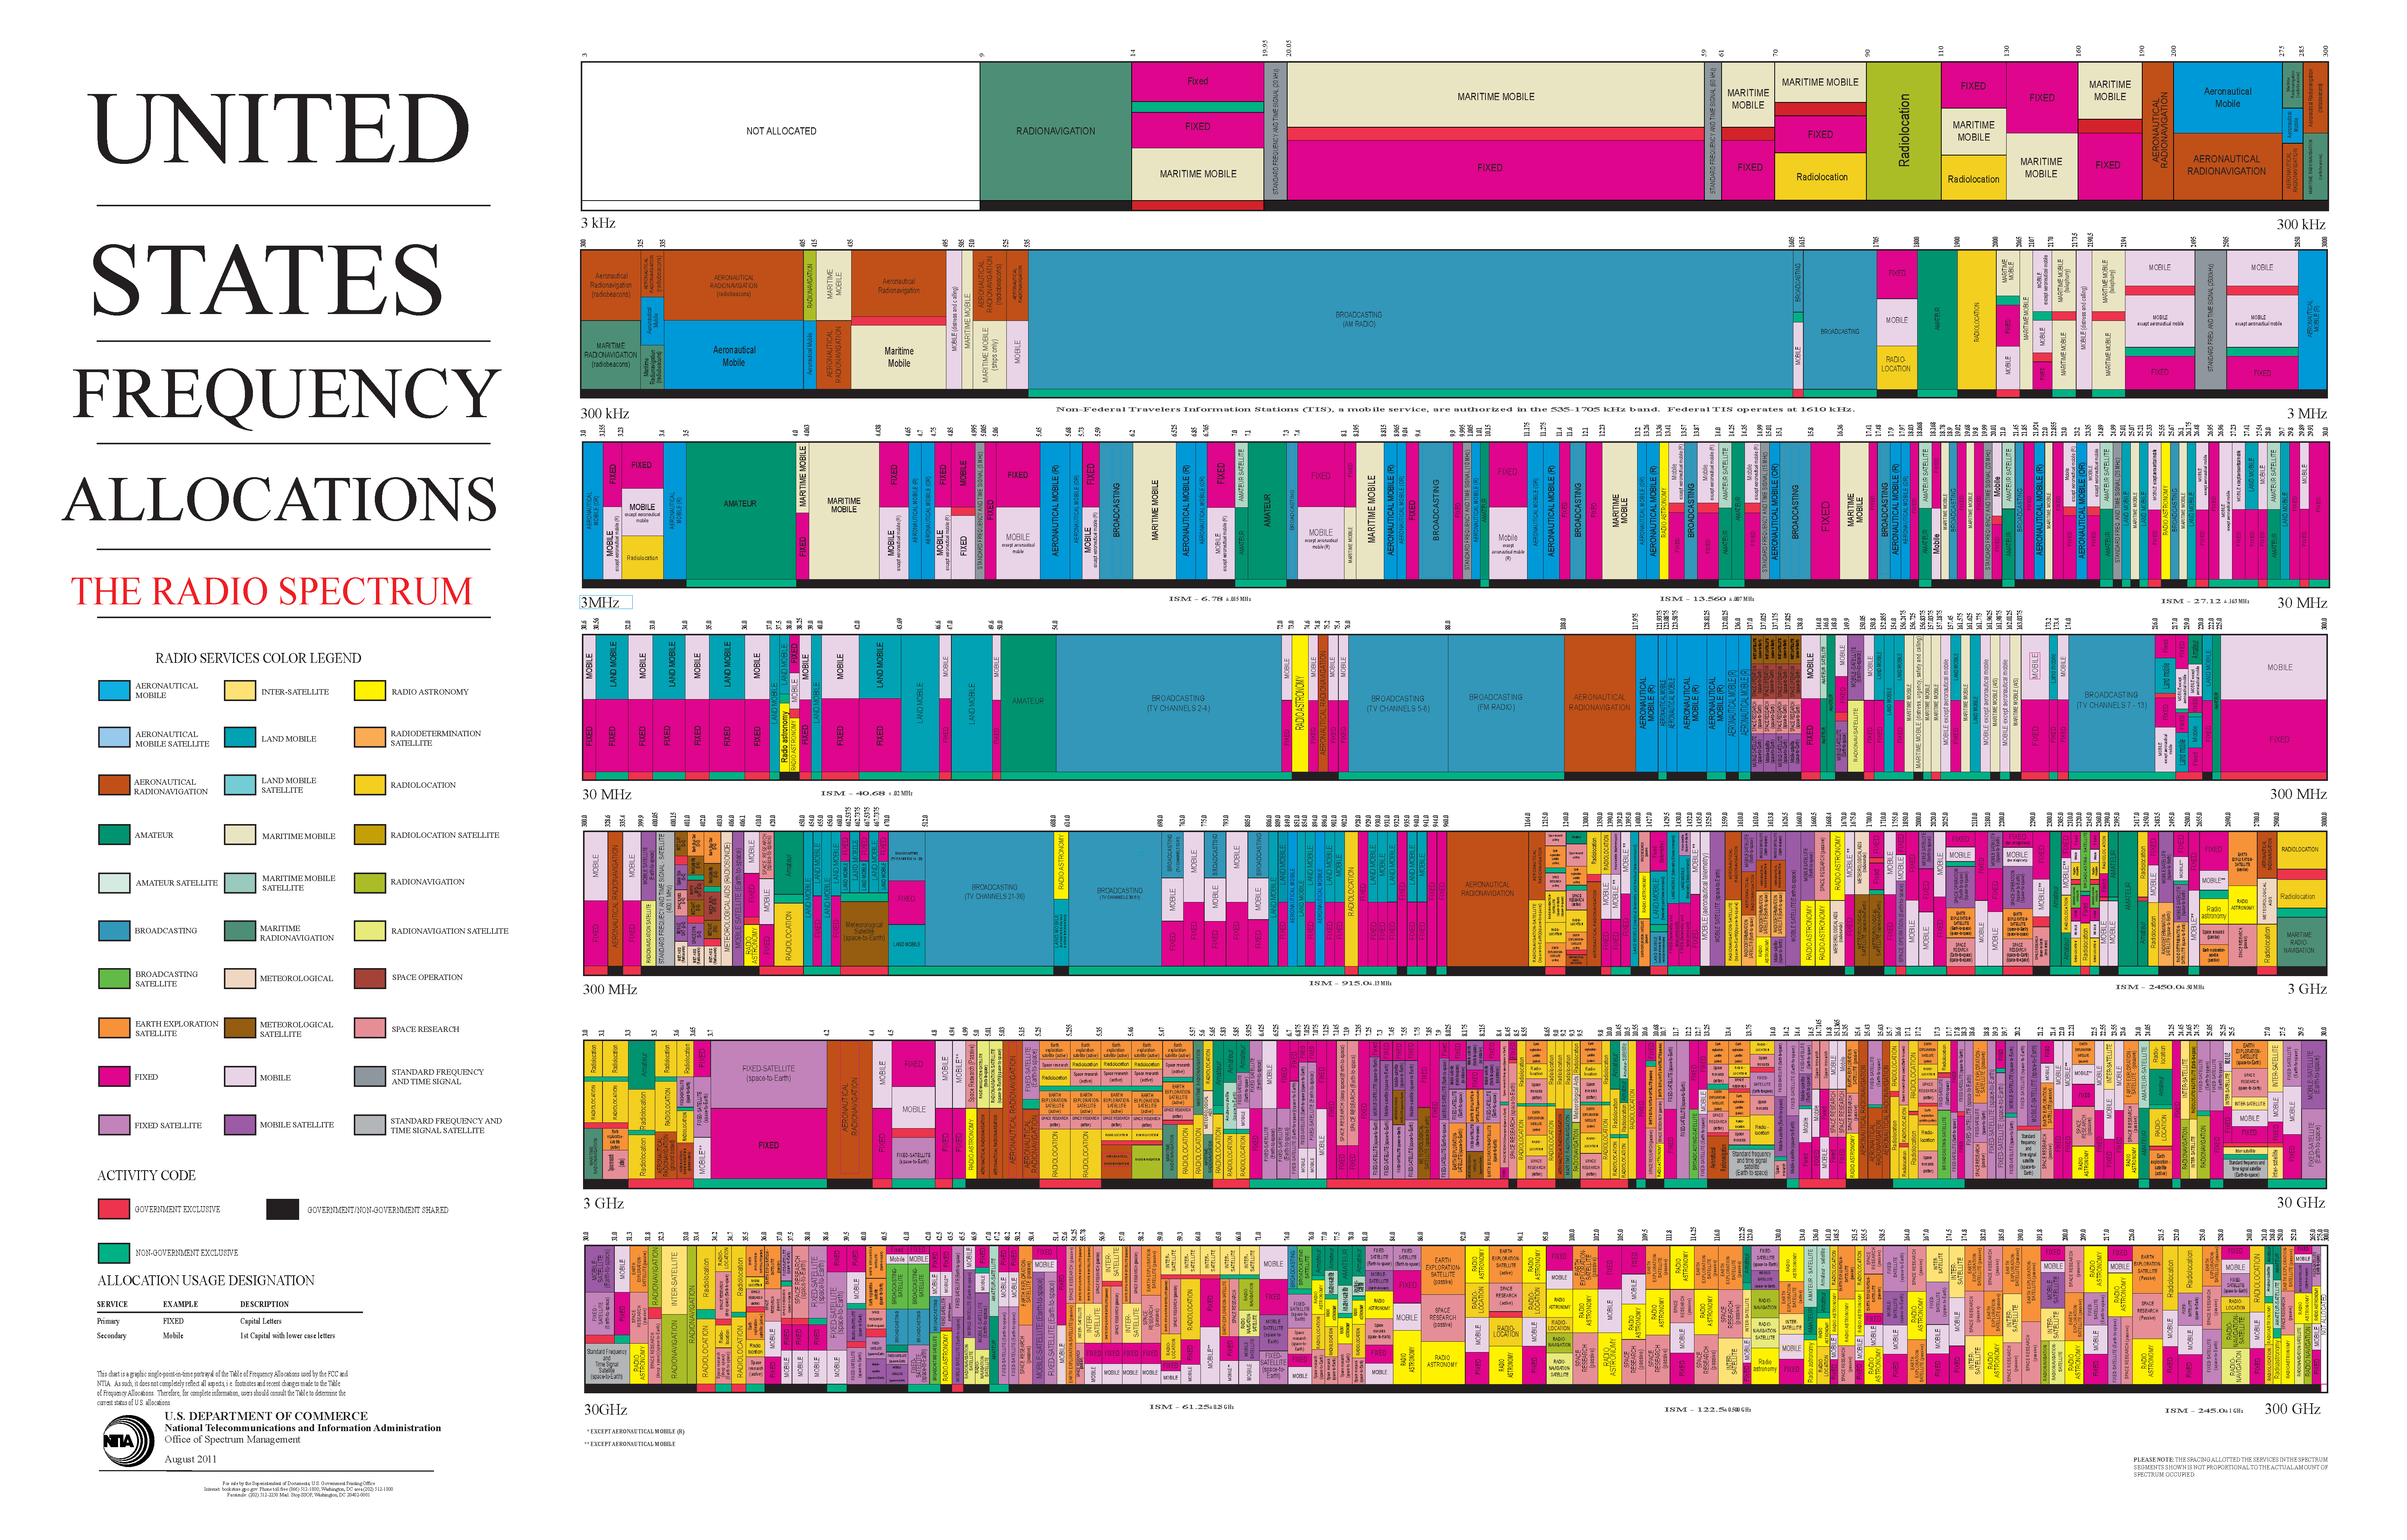
\includegraphics[width=1\textwidth]{US_Frequency_Allocations_Chart.pdf}
	\small    
    \caption{US frequency allocations of the radio spectrum}    
\end{figure}
}
\end{frame}

\begin{frame}{Introduction} \pause
An optional solution: \pause
\bigskip

{\it Cognitive Radio} (CR) - A dynamically configured transceiver. \pause

\bigskip
\begin{itemize}[label=\color{cyan} {$\blacktriangleright$}]
\item First published by Mitola, J. \& Maguire, G.Q., Jr. (1999). \pause
\medskip
\item Haykin, S. (2005) addresses three fundamental cognitive tasks: \pause\smallskip
	\begin{itemize}[label=\color{cyan} {$\triangleright$}]
	\item Radio-scene analysis. \pause\smallskip
	\item Chanel-state estimation and predictive modeling. \pause\smallskip
	\item \textbf{Transmit-power control and dynamic spectrum management.}
	\end{itemize}
\end{itemize}
\end{frame}

\begin{frame}{Introduction} \pause
\begin{itemize}[label=\color{cyan} {$\blacktriangleright$}]
\item Many researches have associated CR with ``Rational Queueing''. \pause\bigskip
\item Do, C. T. {\it et al.} (2012) solve a generalization of Edelson \& Hildebrand's Unobservable Model with server's breakdowns for spectrum sharing in CRN. \pause\bigskip
\item Habachi, O. \& Hayel, Y. (2012) discuss a rather general model of opportunistic sensing, but with no regard to failed-sensing consequences.\bigskip
\end{itemize}
\end{frame}

\begin{frame}{System-Model} \pause
Two identical servers, $S_Q$ and $S_L$, and a single queue. \pause

\bigskip
Customers choose between two options: {\it Sense} $S_L$ or {\it Join} $S_Q$. \pause

\bigskip
\visible<4>{\begin{figure}[h!]
    \centering
    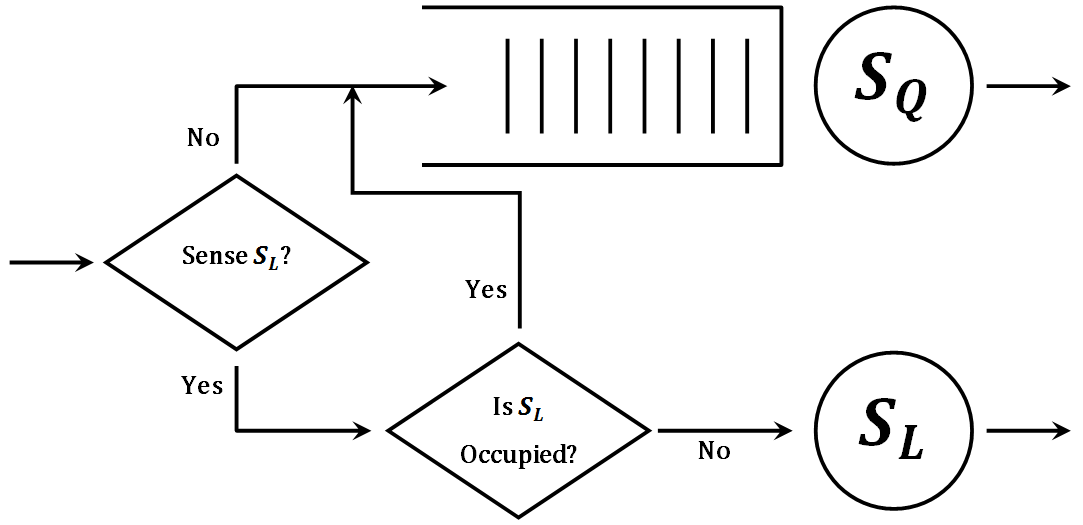
\includegraphics[width=1\textwidth]{../plots/Model.png}
    \small
    \caption{Customers' flow chart of the system }
    \normalsize
\end{figure}}

\end{frame}

\begin{frame}{System-Model} \pause
Formulation: \pause
\bigskip
\begin{itemize}[label=\color{cyan} {$\blacktriangleright$}]
\item Identical rational individualistic customers\pause
\medskip
\item Arrival rate $\sim {\rm Poisson}(\Lambda)$ \pause
\medskip
\item Service duration $\sim {\rm Exp}(\mu)$ \pause
\medskip
\item $p$ - sensing probability \pause
\medskip
\item $(X(t), Y(t))$ - the state at time $t$, where\\ \smallskip
$X(t) \in \lbrace0, 1, 2, \ldots\rbrace$ and $Y(t) \in \lbrace0, 1\rbrace$ \pause
\medskip
\item $P_{i,j}$ - the stationary probability of state $(i,j)$
\end{itemize}
\end{frame}

\begin{frame}{System-Model} 
\visible<2>{\begin{figure}[h!]
    \centering
    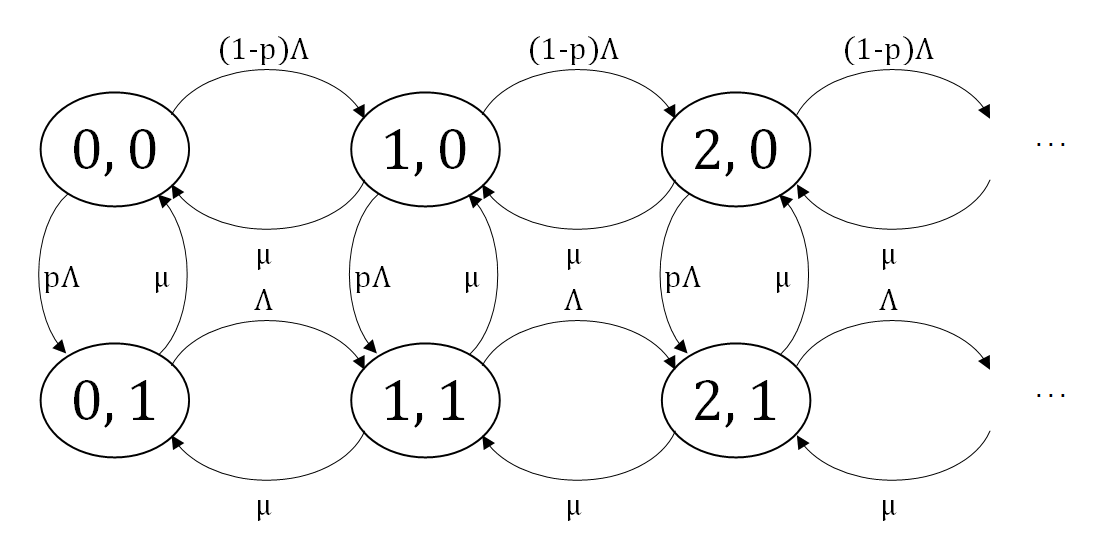
\includegraphics[width=1\textwidth]{../plots/MarkovChain.png}
    \small
    \caption{The Markov chain describing the transitions between states in the system}
    \normalsize
\end{figure}}
\end{frame}

\begin{frame}{System-Model} \pause

This is a particular case of the {\it Heterogeneous Arrivals \& Service} model of Yechiali, U. \& Naor, P. (1971). \pause
\medskip
\\$S_L$ is an independent M/M/1/1 \pause
\medskip
\\The stationary probabilities are found solving the set of equations: \pause
\begin{equation}
  \begin{cases}
    \Lambda P_{0,0} - \mu P_{1,0}  - \mu P_{0,1} = 0\:,\\
    (\mu+\Lambda) P_{0,1} - p\Lambda P_{0,0}  - \mu P_{1,1} = 0\:.
  \end{cases}
	\label{StateEq1}
\end{equation} \pause
and $\forall n \in \lbrace 1, 2, \ldots \rbrace$: \pause
\small
\begin{equation}
  \begin{cases}
    (\mu+\Lambda) P_{n,0} - (1-p) \Lambda P_{n-1, 0} - \mu P_{n+1,0}  - \mu P_{n,1} = 0\:,\\
    (2\mu+\Lambda) P_{n,1} - p\Lambda P_{n,0}  - \Lambda P_{n-1,1} - \mu P_{n+1,1} = 0\:.
  \end{cases} \label{StateEq2}
\end{equation}
\normalsize
\end{frame}

\begin{frame}{System-Model} \pause
Defining $\rho := \sfrac{\Lambda}{\mu}$, after some development we achieve the following results: \pause
\begin{equation}
	\pr(Y=1) = \sum\limits_{i=0}^{\infty} P_{i, 1} = \dfrac{p\rho}{1+p\rho}\:; \label{LossProb}
\end{equation}\pause
\begin{equation}
	\pr(Y=0) = 1-\pr(Y=1) = \sum\limits_{i=0}^{\infty} P_{i, 0} = \dfrac{1}{1+p\rho}\:; \label{OMLossProb}
\end{equation}\pause
\begin{equation}
\begin{split}
	\hat{\rho}(p,\rho) :=& \frac{1}{\mu} \left[ (1-p)\Lambda + \pr(Y=1)\cdot p \Lambda \right] \\  =& \rho - \frac{1}{1+p\rho}p\rho = 1-(P_{0,0}+P_{0,1}) \:.
\end{split}\label{rho hat}
\end{equation}
\end{frame}

\begin{frame}{System-Utilization} \pause
\begin{proposition}\pause
For each $\rho\in(0,\varphi)$, there exists a lower bound for $p$, denoted $\underline{p}$, such that the system is stable iff $p \in (\underline{p}, 1]$. 
\end{proposition} \pause
\begin{proof}\pause
For stability we demand $\hat{\rho}(p,\rho) < 1$. \pause \\ 
Using (\ref{rho hat}) and isolating $p$ in the inequality we get:
\[ p > \frac{\rho - 1}{\rho(2-\rho)} =: \underline{p}\] \pause
By the monotonicity of $\hat{\rho}(p,\rho)$, we assume $p=1$ concluding that
\[ \hat{\rho}(1,\rho)=\frac{\rho^2}{1+\rho}<1 \quad\Leftrightarrow\quad \rho < \frac{1+\sqrt{5}}{2}=\varphi \] 
\end{proof}
\end{frame}

\begin{frame}{Equilibrium Strategy} \pause
We assume $\rho<\varphi$ and define:\pause\\
\medskip
\begin{itemize} [label=\color{cyan} {$\blacktriangleright$}]
\item $c_{w}>0$ - the waiting cost per unit time.\pause\\
\item $c_{s}>0$ - the cost of sensing.\pause\\
\end{itemize}
\medskip
We denote $\gamma :=\sfrac{c_{w}}{\mu c_{s}}$ and write down the costs:\pause
\begin{equation}
\begin{cases}
 	C_{N}(p) = \frac{c_{w}}{\mu}\e\left[L(p)\right] \:; \\
	C_{S}(p) = c_{s} + \pr(Y=1) \cdot \frac{c_{w}}{\mu} \e\left[L(p)\mid Y=1\right] \:;
\end{cases}
\end{equation}\pause
\begin{equation}
\Leftrightarrow
\begin{cases}
 	\frac{1}{c_s}C_{N}(p) = \gamma\e\left[L(p)\right] \:; \\
 	\frac{1}{c_s}C_{S}(p) = 1 + \pr(Y=1) \cdot \gamma \e\left[L(p)\mid Y=1\right] \:.
\end{cases}
\end{equation}
\end{frame}

\begin{frame}{Equilibrium Strategy} \pause
\begin{proposition}\pause For every $\rho\in(0,\varphi)$, and for every value $\gamma>0$, a unique equilibrium strategy $p_{e}\in[0,1]$ exists.
\end{proposition}\pause
\medskip
This result arises in spite of the fact that the function $C_S(p)$ is not necessarily monotone:\pause
\visible<5>{\begin{columns}
\begin{column}{0.5\textwidth}
	\begin{figure}
		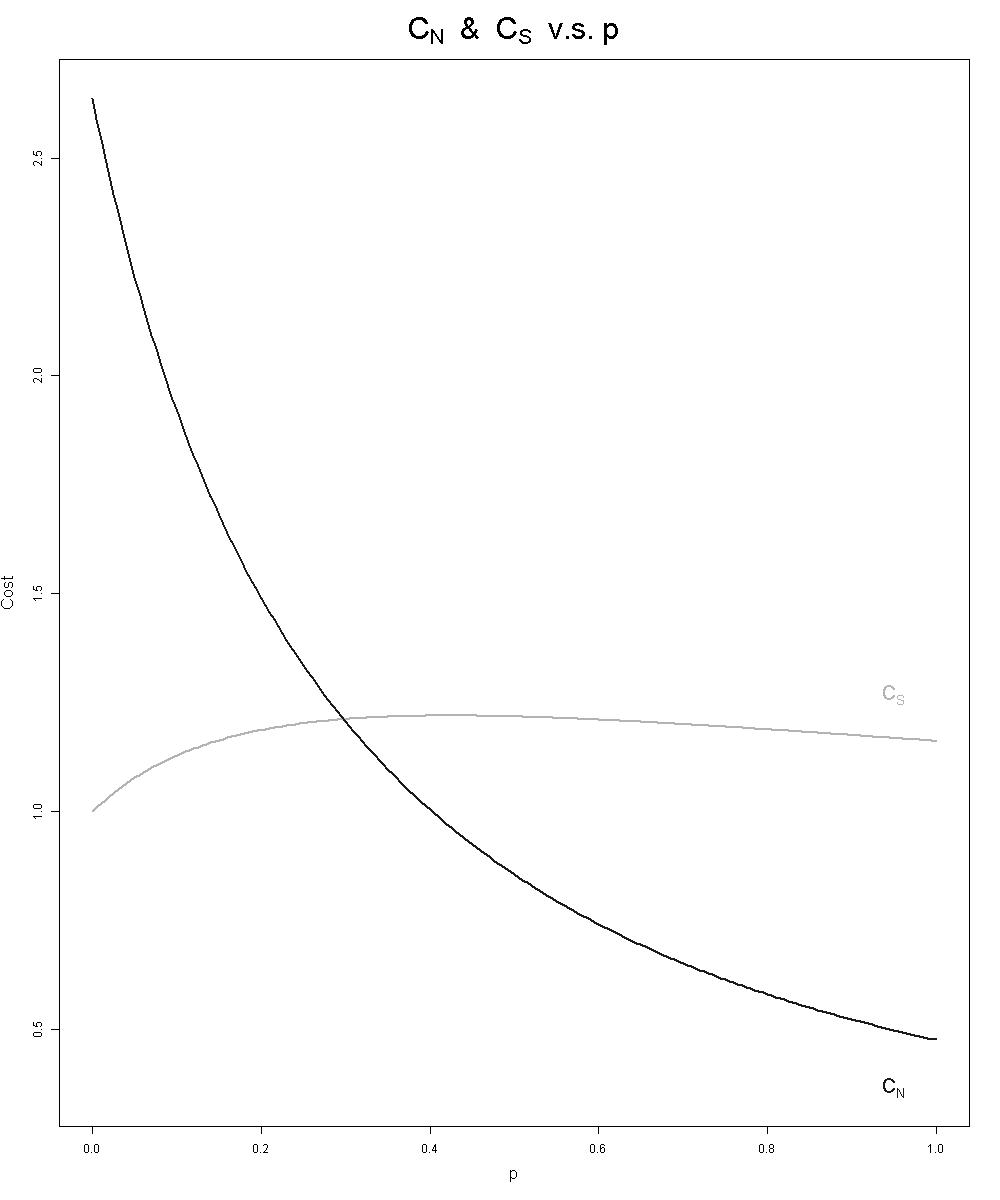
\includegraphics[width=0.7\textwidth]{../plots/cost_vs_p_1_0_725.png}    
		\small
		\caption{$\gamma=1$ and $\rho=0.725$}    
		\normalsize
	\end{figure}
\end{column}

\begin{column}{0.5\textwidth}
	\begin{figure}
		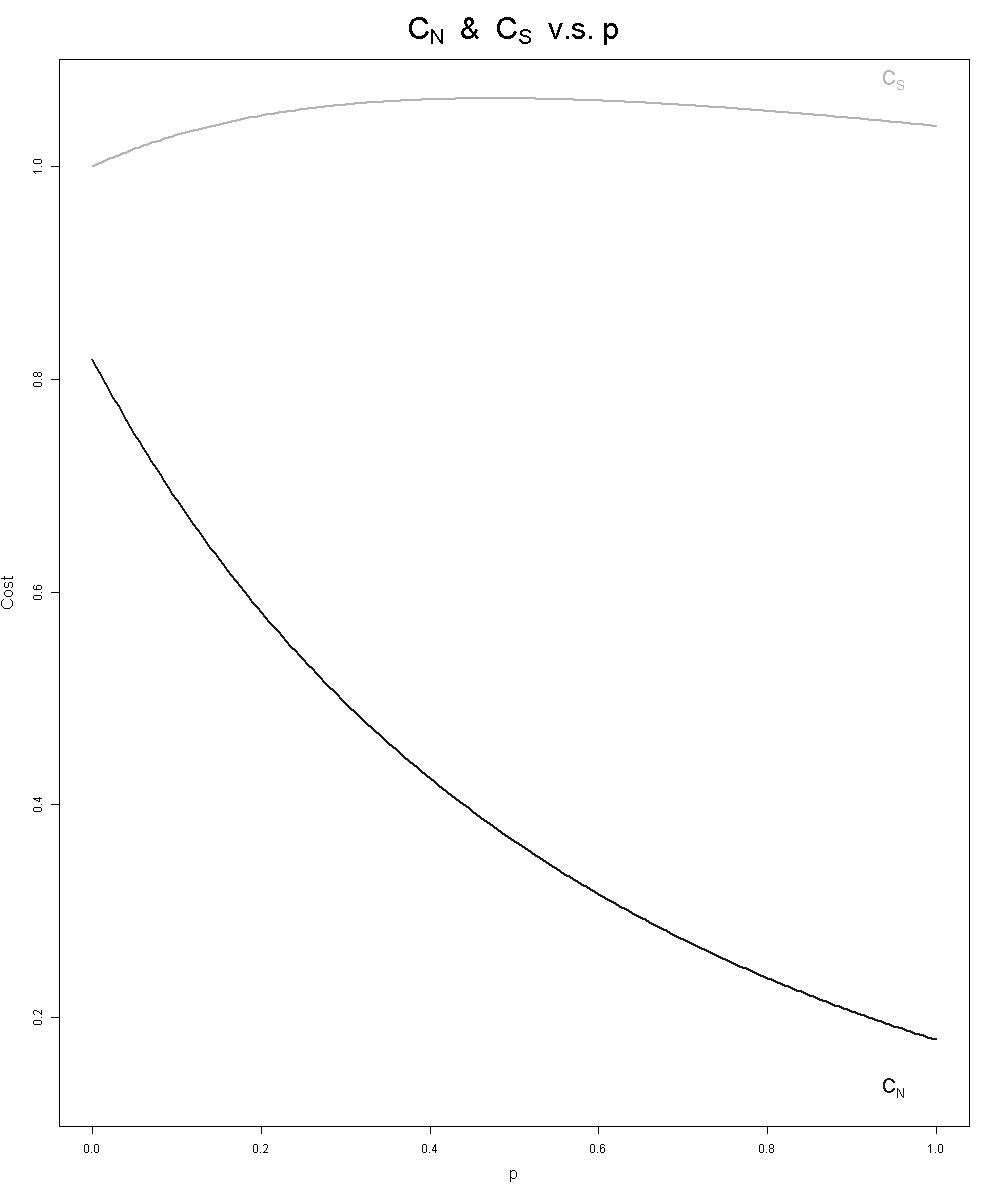
\includegraphics[width=0.7\textwidth]{../plots/cost_vs_p_1_0_45.png}    
		\small		
		\caption{$\gamma=1$ and $\rho=0.45$}    
		\normalsize
	\end{figure}
\end{column}
\end{columns}}

\end{frame}

\begin{frame}{Equilibrium Strategy} \pause
In equilibrium, it must hold that $C_S(p)=C_N(p)$, or equivalently: \pause
\begin{equation}
\gamma \e\left[L(p)\mid Y=0\right] = \frac{1}{\Pr(Y=0)} = 1+p\rho\:.  \label{gamma*e0=1+p*rho}
\end{equation} \pause

\begin{proposition} \pause
The function $\e\left[L(p)\mid Y=0\right]$ is continuous and monotone non-increasing in $p$. \label{MonotonicityProp}
\end{proposition} \pause
\medskip
To prove this we use the Sample Path Analysis technique, comparing two systems under the same sequence of events. \pause
\bigskip

This property together with (\ref{gamma*e0=1+p*rho}) immediately indicate that $p_e$ is unique.

\end{frame}

\begin{frame}{Equilibrium Strategy} \pause
\begin{proofs} \pause
\medskip
Define: \pause
\begin{itemize} [label=\color{cyan} {$\blacktriangleright$}]
	
	\item System $\Omega = \lbrace S_Q, S_L, p \rbrace$ with the state $(X(t), Y(t))$ \pause
		
	\item System $\Omega' = \lbrace S'_Q, S'_L, p' \rbrace$ with the state $(X'(t), Y'(t))$ \pause
		
	\item $\lbrace{ (T_i, \tau_i, u_i) \rbrace}_{i \in \mathbb{N} }$ and $\forall i \in \mathbb{N}:$ \pause
	\begin{itemize} [label=\color{cyan} {$\triangleright$}]
	\item $T_{i+1} - T_i \sim \expdist(\Lambda) \:;$ \pause 
	\item $\tau_i \sim \expdist(\mu) \:;$ \pause
	\item $u_i \sim \U[0,1] \:.$ \pause
	\end{itemize}		
\end{itemize}
\medskip
Assume, w.l.o.g that \pause
\begin{itemize} [label=\color{cyan} {$\blacktriangleright$}]
\item $p < p'$ \pause
\item $(X(0), Y(0)) = (X'(0), Y'(0)) = (0,0)$ \pause
\end{itemize}
\medskip
We shall show: \pause
\[ \e[X' \mid Y'=0] \leq \e[X \mid Y=0] \:. \]
\end{proofs}
\end{frame}

\begin{frame}{Equilibrium Strategy} \pause
\begin{proofs}[\proofname\ (Cont.)] \pause
\medskip
We apply the following modifications: \pause
\begin{enumerate}[label=(\roman*)]
\item\label{Assump1} If $Y(T_i)=1$ (or $Y'(T_i)=1$), customer $i$ preempts the one in service, and the preempted customer is routed to $S_Q$ (or $S'_Q$). \pause
\item\label{Assump2} Subsystem $S_Q$ (or $S'_Q$) is a preemptive resume LCFS queue. \pause
\end{enumerate}

\visible<6>{\begin{figure}[h!]
    \centering
    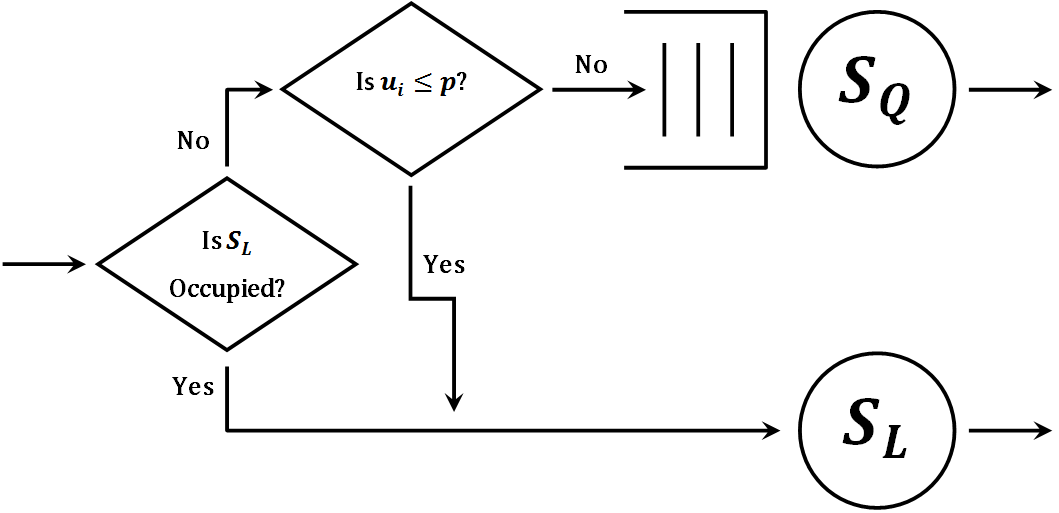
\includegraphics[width=.6\textwidth]{../plots/Model_modif.png}
    \small
    \caption{Customers' flow chart of the modified system }
    \normalsize
\end{figure}}

\end{proofs}
\end{frame}

\begin{frame}{Equilibrium Strategy} \pause 
\begin{proofs}[\proofname\ (Cont.)] \pause
\smallskip
\begin{enumerate}[label=(\alph*)]
\item<3->\label{Prop1} If there is a customer in $S_L$ (or $S'_L$), it must be the last customer.
\item<4->\label{Prop2} Customers $i$ begins service at $T_i$.
\item<5->\label{Prop3} Joining $S_L$ $\Rightarrow$ Joining $S'_L$ 
\[ \forall t  \in [0, \infty): \lbrace{ Y(t)=1 \rbrace} \Rightarrow \lbrace{ Y'(t)=1 \rbrace} \:;\]
\item<6->\label{Prop4} Joining $S'_Q$ $\Rightarrow$ Joining $S_Q$ 
\[ \forall t  \in [0, \infty): \lbrace{ Y'(t)=0 \rbrace} \Rightarrow \lbrace{ Y(t)=0 \rbrace} \:; \] 
\item<7->\label{Prop5} The sojourn time in $S'_Q$ $\leq$ The sojourn time in $S_Q$
\end{enumerate}
\end{proofs}
\end{frame}

\begin{frame}{Equilibrium Strategy} \pause
\begin{proofs}[\proofname\ (Cont.)]\pause
\medskip
From \ref{Prop4} + \ref{Prop5}, \pause
\begin{equation}
\forall t \in [0, \infty):  X(t) \geq X'(t) \:; \quad \mbox{or,} \quad X \succcurlyeq X'\:; \label{StDomination}
\end{equation}\pause
In fact,
\[ \e[X' \mid Y'=0] \leq \e[X \mid Y'=0] \:, \] \pause
and it is left to prove
\[ \e[X \mid Y'=0] \leq \e[X \mid Y=0] \:. \] \pause
Note that for some $\lambda_1, \lambda_2 \in [0,1]$ s.t. $\lambda_1+\lambda_2=1$: \pause
\begin{equation}
	\e_{Y=0}[X] \: = \: \lambda_1 \e[X \mid Y'=0] \: +\: \lambda_2 \e_{Y=0}[X \mid Y'=1] \:. \label{convex comb.}
\end{equation}
\end{proofs}
\end{frame}

\begin{frame}{Equilibrium Strategy} \pause
\begin{proof}[\proofname\ (Cont.)] \pause
\medskip
In the paper we show explicitly that
\[ \e_{Y=0}[X] \leq \e_{Y=0}\left[ X \left| \: \parbox[h]{1.8cm}{ \begin{small} busy period \\ has begun \end{small}} \right. \right] = \e_{Y=0}[X \mid Y'=1] \:, \] \pause
which, alongside (\ref{convex comb.}) implies that
\[ \e[X \mid Y'=0] \leq \e_{Y=0}[X] \leq \e_{Y=0}[X \mid Y'=1] \:, \] \pause
to complete the proof of the proposition.
\end{proof}
\end{frame}

\begin{frame}{Equilibrium Strategy} \pause
\begin{proposition} \pause
The pure strategy $p=0$ is an equilibrium strategy (in other words $p_e=0$) iff:
\[ \rho \leq \frac{1}{1+\gamma} \:.\]
\end{proposition} \pause
\begin{proof} \pause
\medskip
This is immediate, as $p=0$ is the M/M/1 regular case and
\[ \e[L(0)\mid Y=0] = \e[L(0)] = \frac{\rho}{1-\rho} \:.\] \pause
Substituting this in (\ref{gamma*e0=1+p*rho}) and isolating $\rho$ we get the desired result.
\end{proof}
\end{frame}

\begin{frame}{Equilibrium Strategy} 
\visible<2>{\begin{figure}[h!]
  \centering
    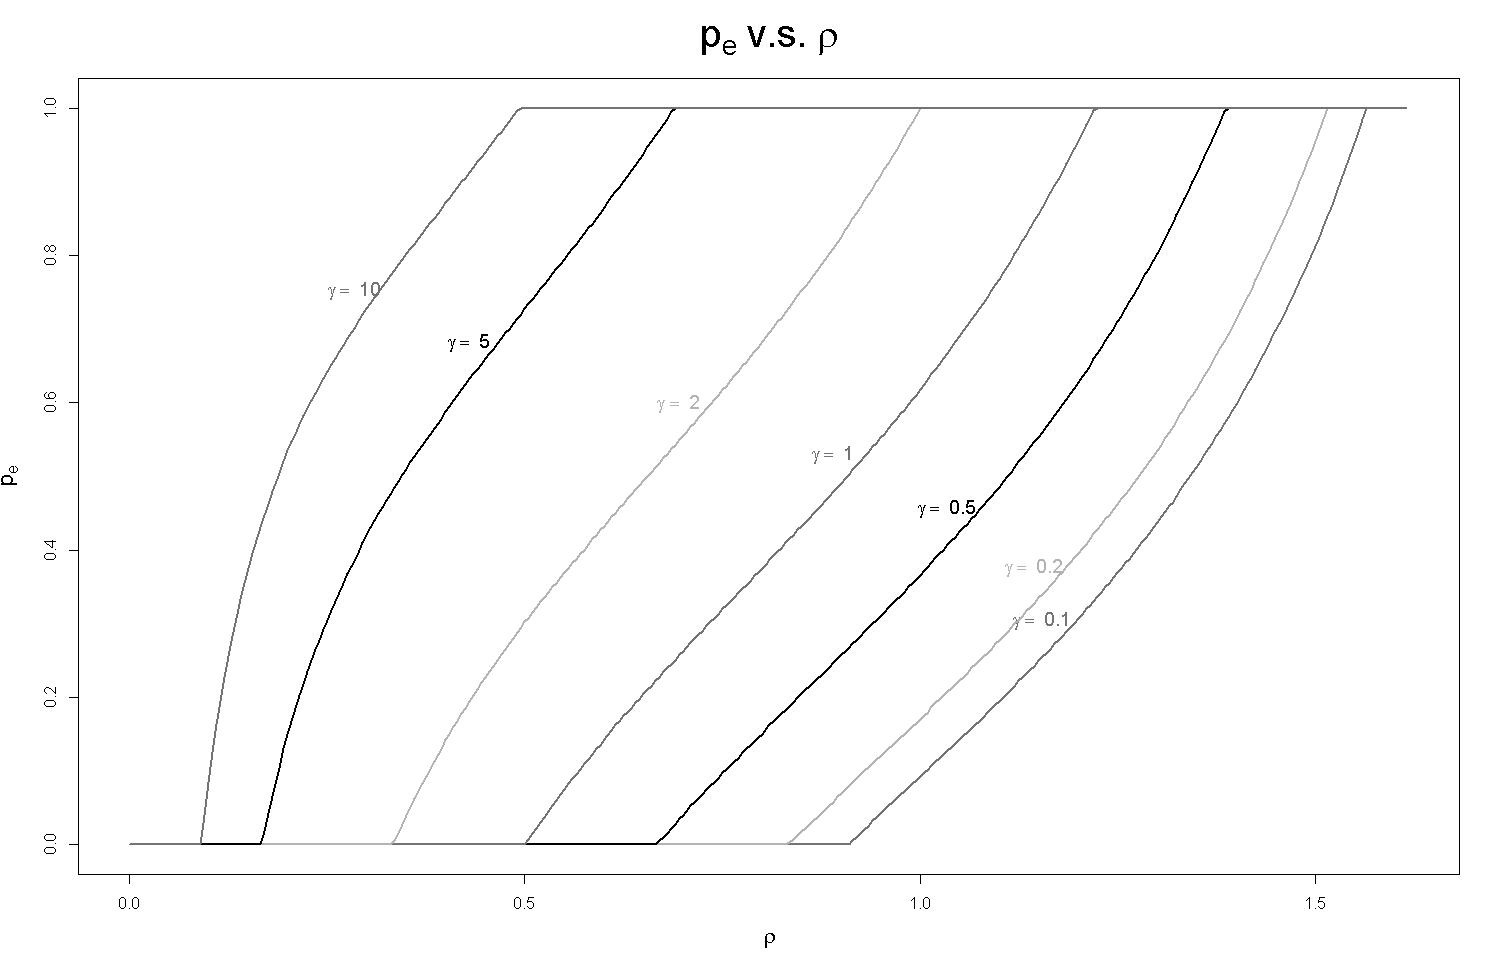
\includegraphics[width=1\textwidth]{../plots/peq_vs_rho.png}
    \caption{The equilibrium strategy $p_{e}$ as a function of $\rho$ for a various values of $\gamma$}
    \label{PeqVsRho}
\end{figure}}
\end{frame}

\begin{frame}{Social Optimization} \pause
The social objective function, $C(p)$, is defined as \pause
\begin{equation}
C(p) := (1-p)C_N(p)+pC_S(p) \:. \label{Cp def.}
\end{equation}\pause
Denote $p^*$ the socially optimal strategy. Accordingly, \pause
\begin{equation}
p^*:=\argmin_{p \in [0,1]}{C(p)}\:.
\end{equation} \pause
and the values can be computed numerically. \pause

\bigskip
For some values of $\rho$ and $\gamma$, we spotted, counter intuitively that $p_e < p^*$.
\end{frame}

\begin{frame}{Social Optimization} \pause
\visible<2>{\begin{columns}
\begin{column}{0.5\textwidth}
	\begin{figure}
		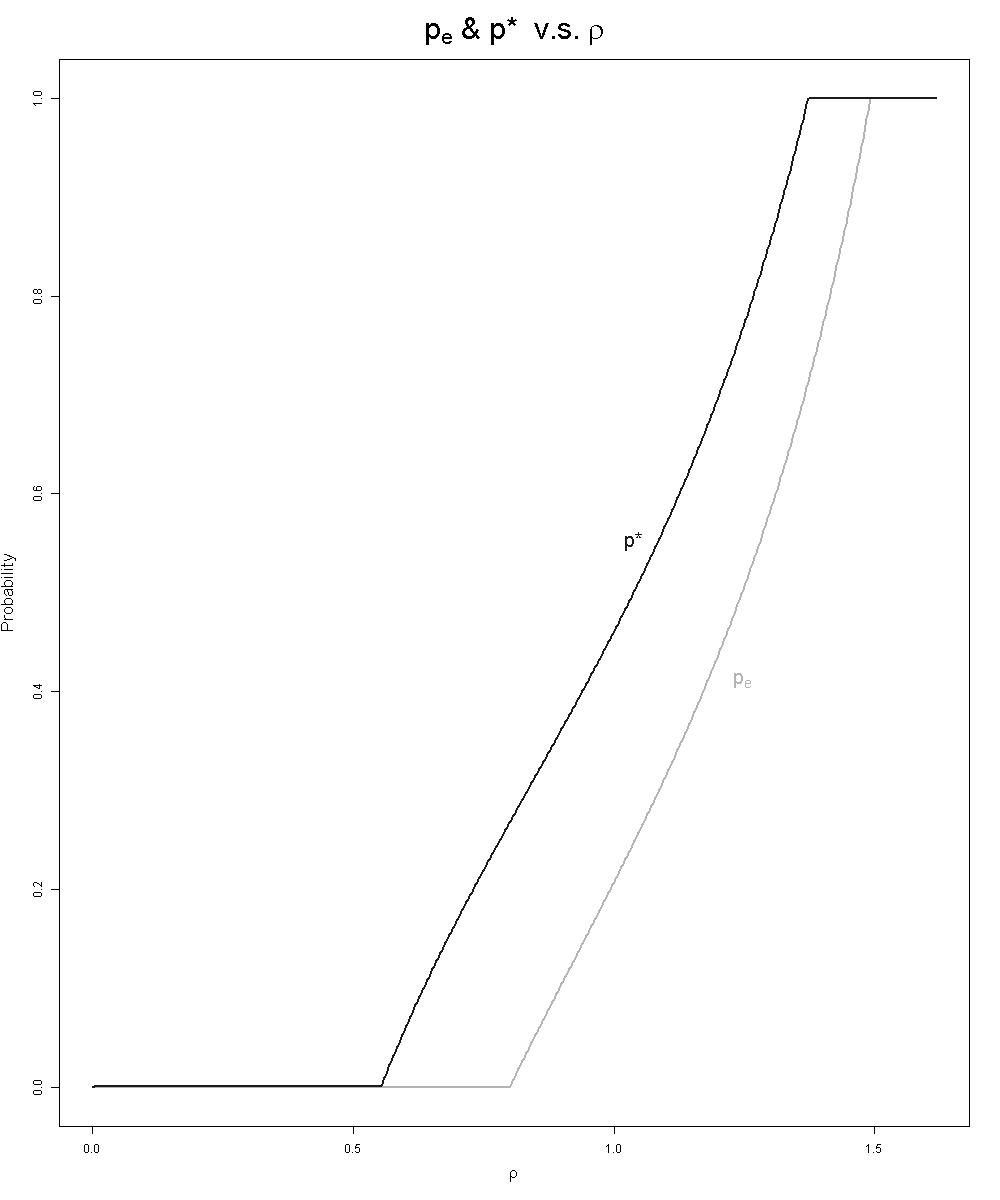
\includegraphics[width=1\textwidth]{../plots/pe_vs_pstar_0_25.png}    
		\small
		\caption{$\gamma=0.25$}    
		\normalsize
	\end{figure}
\end{column}
\begin{column}{0.5\textwidth}
	\begin{figure}
		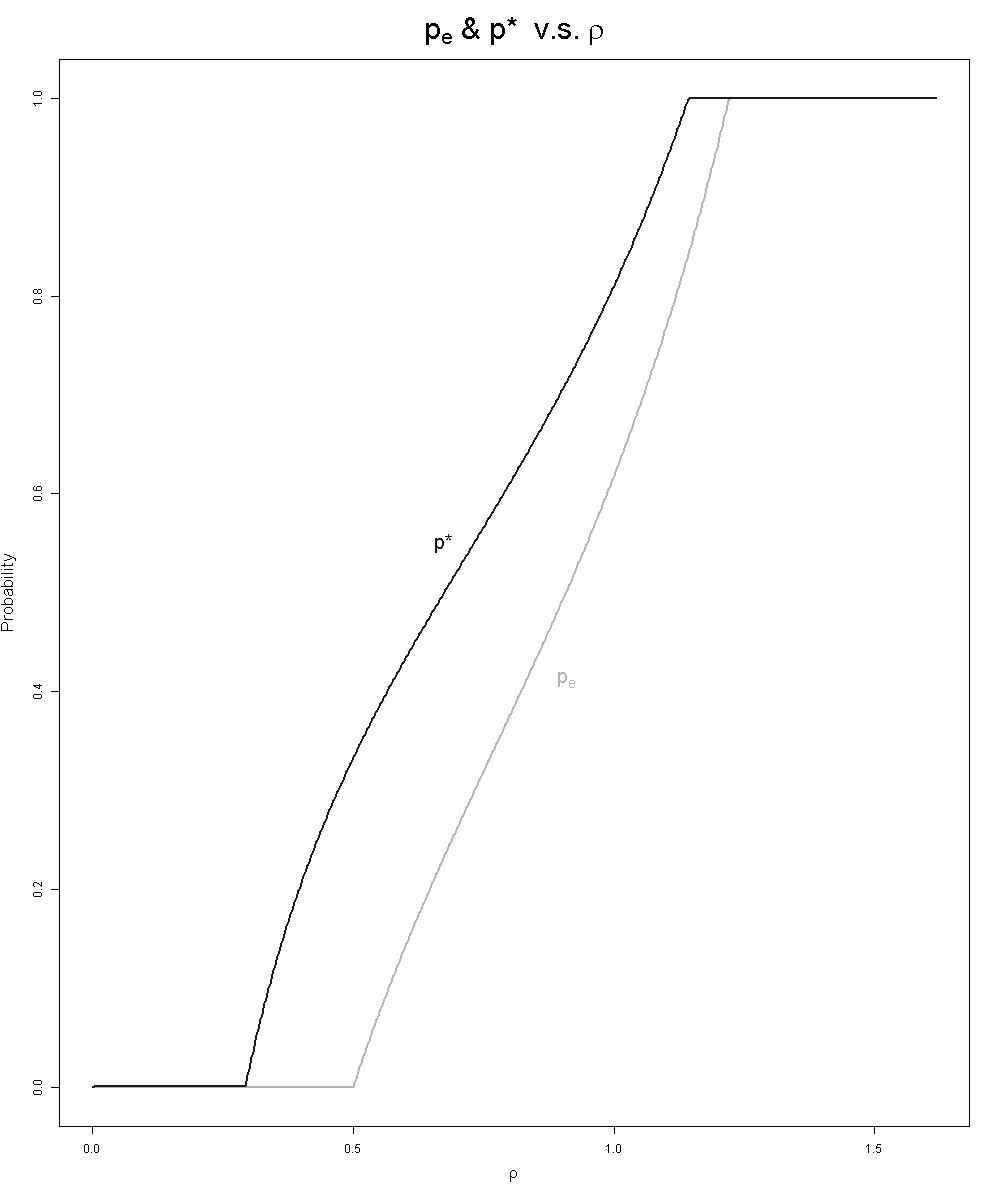
\includegraphics[width=1\textwidth]{../plots/pe_vs_pstar_1.png}    
		\small		
		\caption{$\gamma=1$}    
		\normalsize
	\end{figure}
\end{column}
\end{columns}}
\end{frame}

\begin{frame}{Social Optimization} \pause
\visible<2>{\begin{columns}
\begin{column}{0.5\textwidth}
	\begin{figure}
		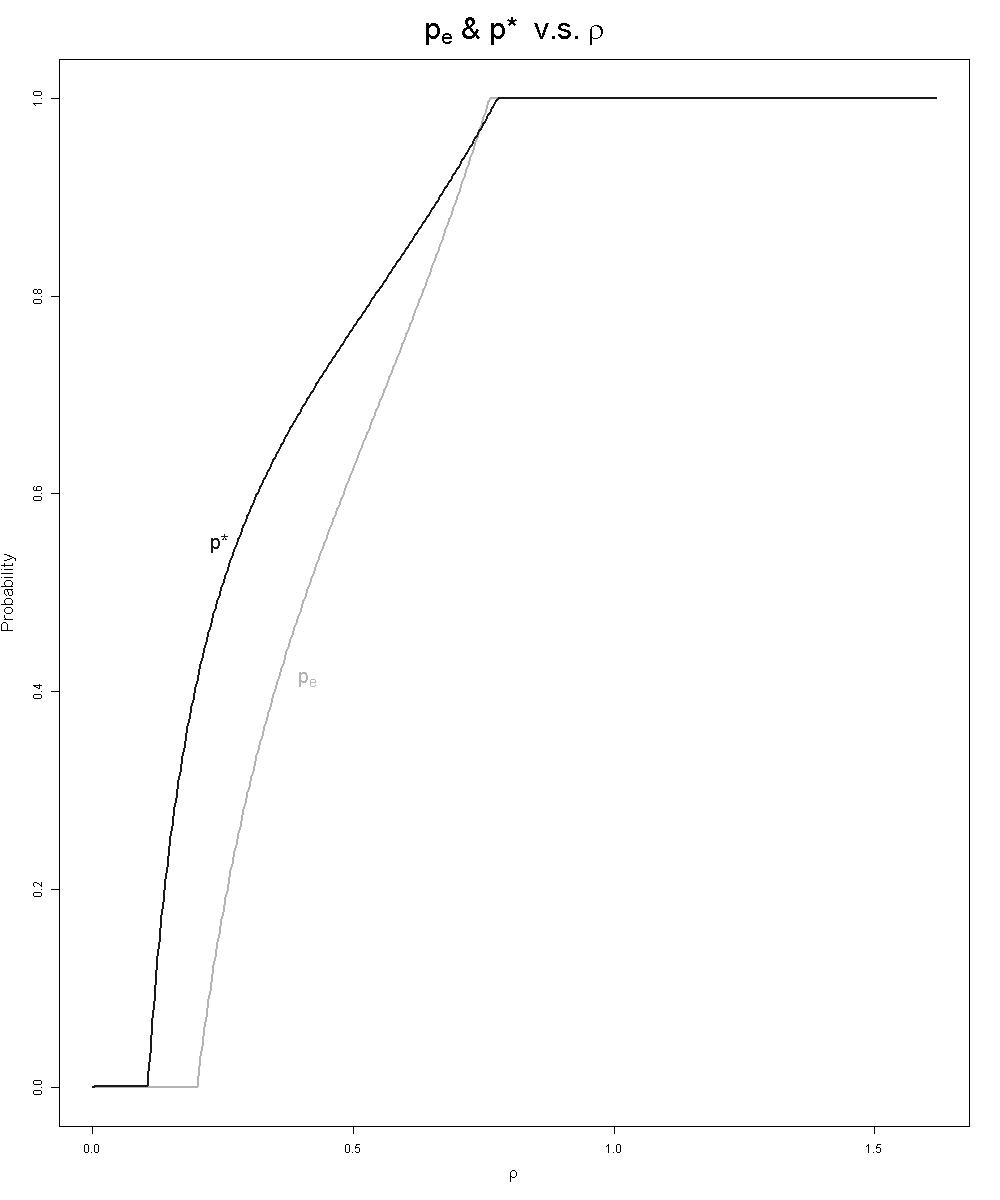
\includegraphics[width=1\textwidth]{../plots/pe_vs_pstar_4.png}    
		\small
		\caption{$\gamma=4$}    
		\normalsize
	\end{figure}
\end{column}
\begin{column}{0.5\textwidth}
	\begin{figure}
		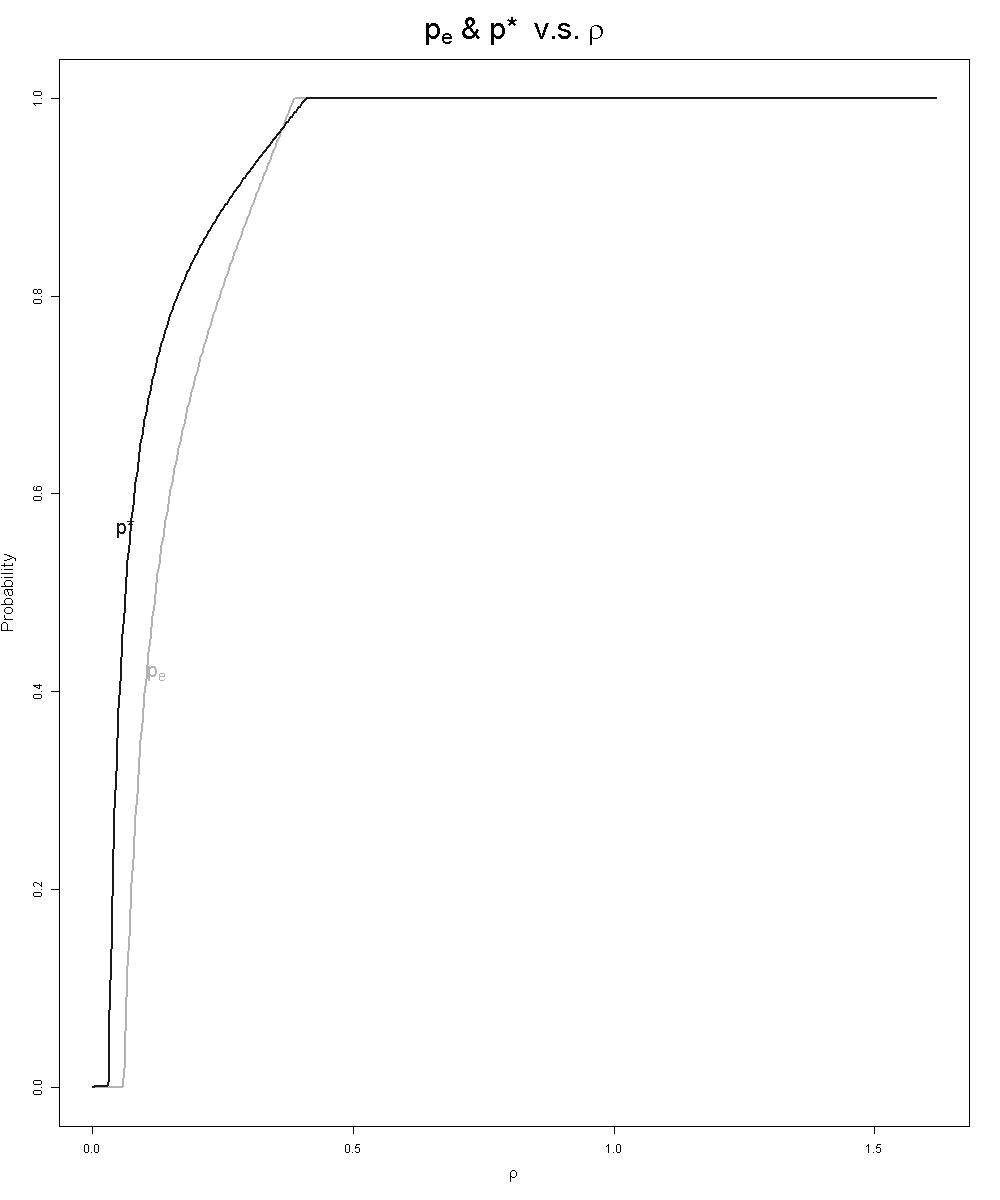
\includegraphics[width=1\textwidth]{../plots/pe_vs_pstar_16.png}    
		\small		
		\caption{$\gamma=16$}    
		\normalsize
	\end{figure}
\end{column}
\end{columns}}
\end{frame}

\begin{frame}{Social Optimization} \pause
\visible<2>{\begin{columns}
\begin{column}{0.5\textwidth}
	\begin{figure}
		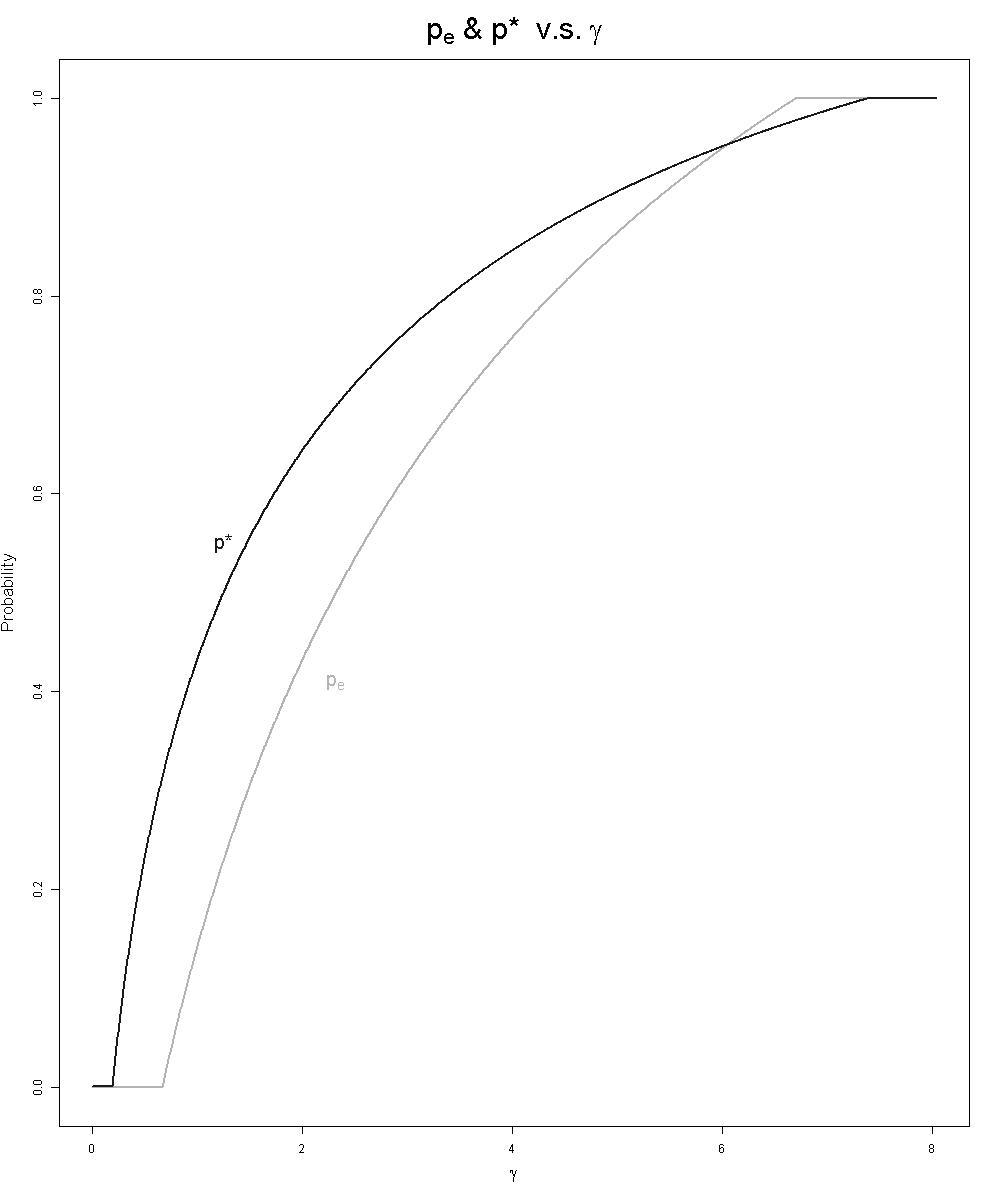
\includegraphics[width=1\textwidth]{../plots/pe_vs_pstar_rev_0_6.png}    
		\small
		\caption{$\rho=0.6$}    
		\normalsize
	\end{figure}
\end{column}
\begin{column}{0.5\textwidth}
	\begin{figure}
		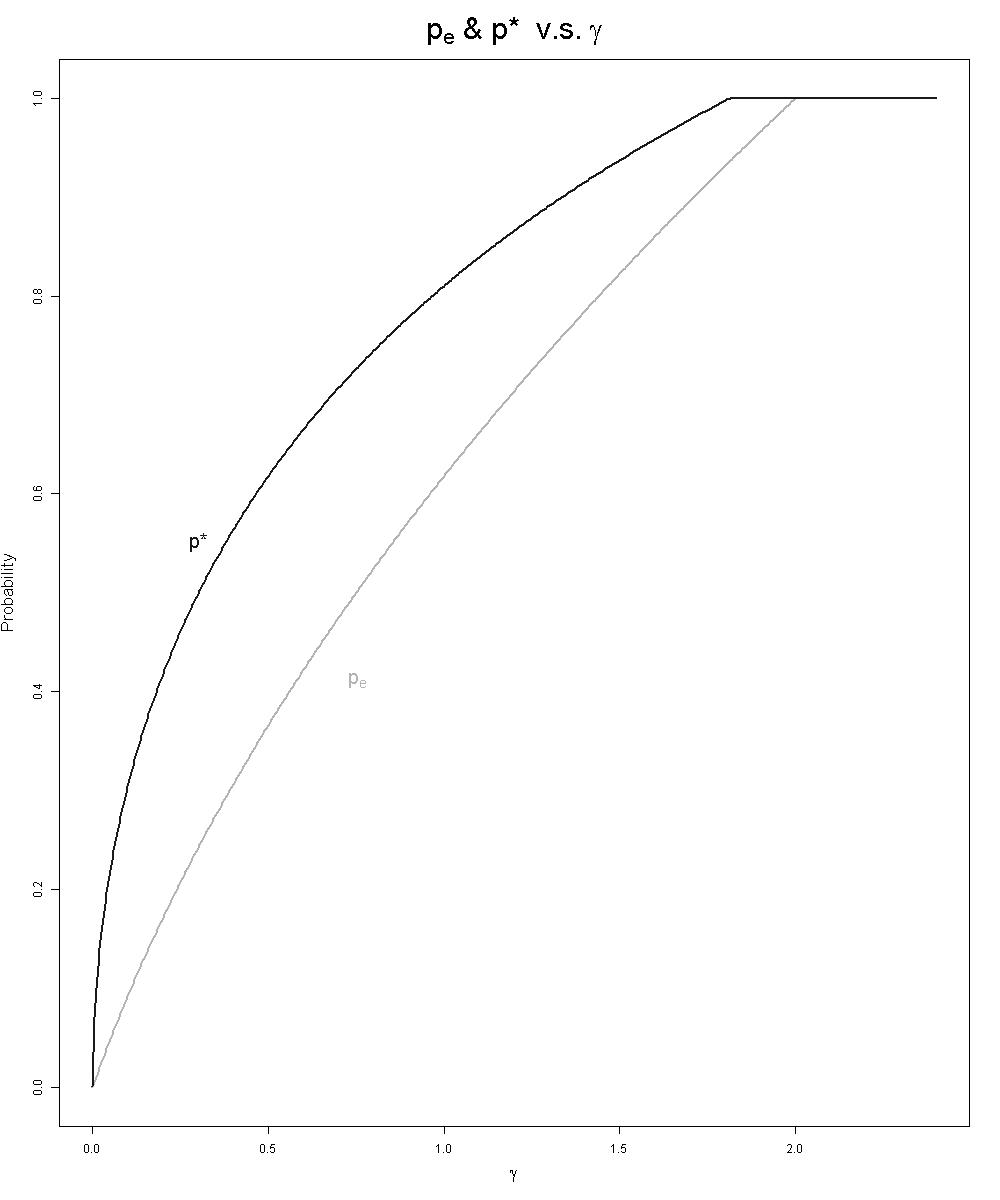
\includegraphics[width=1\textwidth]{../plots/pe_vs_pstar_rev_1.png}    
		\small		
		\caption{$\rho=1$}    
		\normalsize
	\end{figure}
\end{column}
\end{columns}}
\end{frame}

\begin{frame}
\begin{Huge}
\begin{center}
Thank you for listening!
\end{center}

\end{Huge}
\end{frame}

\end{document}